\documentclass[12pt, conference]{IEEEtran}
\IEEEoverridecommandlockouts
% The preceding line is only needed to identify funding in the first footnote. If that is unneeded, please comment it out.
\usepackage{cite}
\usepackage{amsmath,amssymb,amsfonts}
% \usepackage{algorithmic}
\usepackage{graphicx, wrapfig, subcaption}
\usepackage{textcomp}
\usepackage{xcolor}
\usepackage{hyperref}
\usepackage[OT1]{fontenc}
\usepackage{setspace}
% Packages added by me
\usepackage[numbers]{natbib} % Manual of natbib at https://gking.harvard.edu/files/natnotes2.pdf
\usepackage{lipsum}
\usepackage{algorithm}
\usepackage{algpseudocode}

\definecolor{cust-linkcolor}{HTML}{7936ff}

\hypersetup{
    colorlinks=true,
    linkcolor=cust-linkcolor,      
    urlcolor=blue,
    citecolor=red
}

\begin{document}

\title{\textbf{Security Key Authentication for Web Applications}\\
{\small CS588 - Networked Distributed System Security $\mid$ Professor J. Solworth}
% \thanks{Identify applicable funding agency here. If none, delete this.}
}

\author{\IEEEauthorblockN{Davide Giacomini}
\IEEEauthorblockA{\textit{dept. of Engineering} \\
\textit{University of Illinois at Chicago (UIC)}\\
Chicago (IL), USA \\
giacomini.davide@outlook.com}
\\
% \IEEEauthorblockN{Jake Campbell}
% \IEEEauthorblockA{\textit{dept. of Engineering} \\
% \textit{University of Illinois at Chicago (UIC)}\\
% Chicago (IL), USA \\
% jacobpmcampbell@gmail.com}
}

\maketitle
% Those two lines are useful for numbered pages
\thispagestyle{plain}
\pagestyle{plain}
\onehalfspacing

\begin{abstract}
    The U2F (Universal 2nd Factor Authentication) protocol allows you to send a cryptographic challenge to a device (typically a key fob) owned by the user. A password starts the process, but the digital key is required to gain access. The FIDO U2F protocol was developed in 2014, and since then, the standards have been honed, refined, and updated. More users are growing accustomed to the idea of cryptographic keys. Some even demand this protection to keep their data safe and secure.

    In this brief report I will analyze the advantages of using a security key, and I will dive into the cryptographic protocol harnessed by those devices. Finally, I will present a sample web application, aimed at showing how current libraries and APIs can be exploited to ease the development of security key authentication in web applications.
\end{abstract}

\begin{IEEEkeywords}
    web applications, authentication, security key, FIDO, U2F, security
\end{IEEEkeywords}

\section{Introduction}\label{introduction}
In security, three main factors of authentication can be distinguished: \emph{to know}, \emph{to have} and \emph{to be}. The first one requires the user to remember something, usually a password associated to the email or a username. The second one requires the user to own something during authentication, for example their own smartphone, or a physical key. The latter implies to recognize the user based on something that characterizes their uniqueness, for example from a fingerprint or their face.

Although passwords are inherently the weakest form of security to consider, they are actually the most widespread as form of user authentication on the web today \cite{reynolds2018tale}. Several are the techniques used to violate a password-protected account, among them there is phishing, guessing or spoofing \cite{reynolds2018tale}. Therefore, many have advocated for the use of a second factor for authenticating (2FA: 2 Factor Authentication) \cite{bonneau2012quest}, thus limiting guessing and spoofing. Biometric authentication is becoming more and more widespread, especially with fingerprint scanners on phone, and in the last years with face scanner too. There are although several issues still not widely studied in biometric authentication, and systems still have defects that bring to their vulnerability. \citet{bonneau2012quest} surveyed these issues and also considered that some biological features have not been deeply studied yet.

Despite 2FA is extremely effective for better secure accounts, there are still attacks that can be carried out. For instance, OTPs can be victim of the so called real-time phishing attacks, which require the attacker to act as a ``server-in-the-middle'', pretending to be the real server and forwarding user's authentication requests and user's OTP to the real server \cite{reailton2015phishing}. However, message-based OTPs are the most used 2FA nowadays, especially because they rely on the assumption that a user will always carry their smartphone with them.

In this report, I will explain why security keys are theoretically better rather than other 2FA methods common today, bringing up problems in using other second factors and showing how they are avoided with a security key. I will then go through a sample web application that I developed in NodeJS\footnote{\url{https://nodejs.org/en/}} and VueJS\footnote{\url{https://vuejs.org/}}, using Express\footnote{\url{https://expressjs.com/}} as framework, after looked at an overview of the cryptographic protocol used by Yubico\footnote{\url{https://yubico.com}} for their security keys.
\section{Related Work}\label{related-work}
I would like now to report the most relevant related work in second factor authentication. \citet{lang2016security} consulted a variety of excellent surveys work \cite{bonneau2012quest,herley2009passwords,biddle2012graphical,jain2007handbook} and listed five different technologies for 2FA, illustrating how security keys could fill some gaps in security left by those technologies. I will address four of them:
\begin{itemize}
    \item \textbf{One-Time Passcodes:} Though OTPs provide more security than passwords, OTPs have a number of downsides. First, they are vulnerable to phishing and man-in-the-middle attacks, as I cited in Sec. \ref{introduction}. Second, OTPs that are delivered by phones are subject to data and phone availability, while those that are generated by dongles cause the user to have one dongle per web site. Finally, OTPs provide a sub-optimal user experience as they often require the user to manually copy codes from one device to another. \emph{Security Keys are resistant to phishing and man-in-the-middle by design; our preliminary study also shows that they provide a better user experience.}
    \item \textbf{Smartphones as Second Factor:} While leveraging the user’s phone as a cryptographic second factor is promising, it faces a number of challenges: for example, protecting application logic from malware is difficult on a general purpose computing platform. Moreover, a user’s phone may not always be reachable: the phone may not have a data connection or the battery may have run out. \emph{Security keys require no batteries and usually have a dedicated
    tamper-proof secure element.}
    \item \textbf{TLS Client Certificates:} Unfortunately, current implementations of TLS client certificates have a poor user experience. Typically, when web servers request that browsers generate a TLS client certificate, browsers display a dialog where the user must choose the certificate cipher and key length—a cryptographic detail that is unfamiliar and confusing to most users. Accidentally choosing the wrong certificate will cause the user’s identity to leak across sites. TLS client certificates also suffer from a lack of portability: they are tough to move from one client platform to another. \emph{Security Keys have none of these issues: they are designed to be simple to use, portable and fool-proof.}
    \item \textbf{Electronic National Identification Cards:} Some countries have deployed
    national electronic identification cards. Despite their rich capabilities, national identity cards require special hardware (a card reader) and thus are hard to deploy. Moreover, they are by definition
    controlled by one government, which may not be acceptable to businesses in another country and could arise a general concern about user's privacy. \emph{Security Keys have no such downsides: they work with pre-installed drivers over commonly available physical media (USB, NFC, Bluetooth) and are not controlled or distributed by any single entity.}
\end{itemize}
\section{Protocol Overview}
\section{Sample Web Application Implementation}\label{implementation}
I developed a web application harnessing the u2f-ref-code library ``u2f-api.js''\footnote{\href{https://github.com/google/u2f-ref-code/blob/master/u2f-gae-demo/war/js/u2f-api.js}{u2f-api.js}} library developed by Google \cite{lang2016security}. I took advantage of the tutorial of The Polyglot Developer\footnote{\url{https://www.youtube.com/watch?v=9d-mp6_vVUM}} on YouTube, and I used the Express framework for the backend, mentioned in Sec.~\ref{introduction}. I used VueJS for the frontend, harnessing the Caddy framework. I used an old version of Caddy, it does not work if you download the latest. I detailed how to download the necessary and how to setup the sample application on GitHub\footnote{\url{https://github.com/davide-giacomini/u2f-login_yubikey_express}}.

Just as a reminder, this is a sample application. It is not thought to scale for bigger purposes, but it is thought to show how to harness existing libraries to relatively easily develop a security key authentication. Therefore, it does not have a database but it simply stores the user information on a variable that gets overwritten at each registration.

The U2F protocol requires to work on \texttt{https} web pages, hence I also generated a self-generated certificate to work in localhost.

\subsection{Server Side}\label{server}
On the server side, I support four requests: a \textsc{GET} and a \textsc{POST} request for the registration and a \textsc{GET} and a \textsc{POST} request again for the authentication.

I used a library provided by the NodeJS environment called U2F to harness its functions \texttt{request}, \texttt{checkRegistration} and \texttt{checkSignature}. On GitHub there are the details on how to download each library I used.

\subsubsection{Server Registration}\label{server-registration}
See Fig.~\ref{fig:server-registration} for more details. When the user asks for registering a new security key, they perform a \textsc{GET} request to the server. The server will, in turn, use the \texttt{request} function to provide to the client an object with 1. the challenge, 2. the web origin (which is called appId in my application) and 3. the version of the U2F protocol (which in my case is the version 2).

\begin{figure}[h]
    \centering
    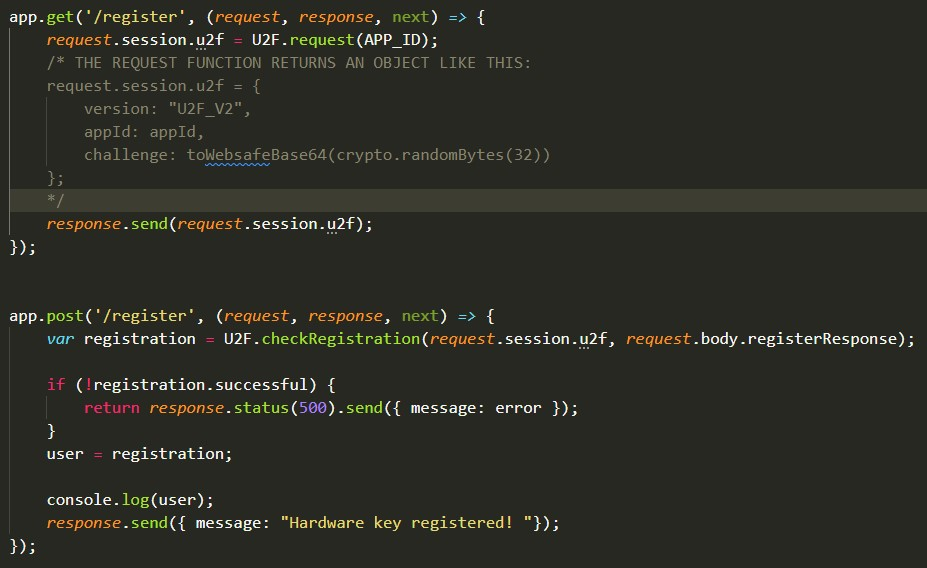
\includegraphics[width=\linewidth]{resources/register-code-server-2.jpg}
      \caption{Server registration code}
      \label{fig:server-registration}
\end{figure}

The Client will forward the information provided by the server to the device, which will generate a key pair and get back to the Client with the information listed in Sec. \ref{registration-protocol}. The security key produces a Registration Message, explained in Sec. \ref{client-registration}, which will be forwarded by the Client to the server. The server will compare the Registration Message (\texttt{registerResponse} in my application) to the object previously sent to the Client to check the presence of man-in-the-middle attacks, as explained in Sec. \ref{registration-protocol}, and, if nothing is wrong, will register the new user in its database.

\subsubsection{Server Authentication}\label{server-authentication}
Refer to Fig.~\ref{fig:server-authentication} for details. The process is very similar to the registration. Now, the server will send the key Handle previously stored along with the other information sent mentioned in Sec. \ref{server-registration}.

\begin{figure}[h]
    \centering
    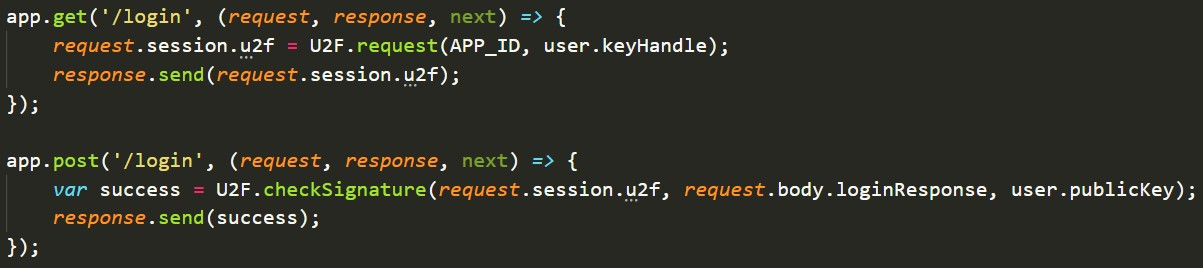
\includegraphics[width=\linewidth]{resources/login-server-code.jpg}
      \caption{Server authentication code}
      \label{fig:server-authentication}
\end{figure}

In turn, the Cient will ask the device to check everything and extract the privat key, as explained in Sec.~\ref{authentication-protocol}. The device will return an Authentication Message, detailed in Sec.~\ref{client-authentication}, to the Client, which will forward it to the server.

Finally, the server will check the signature using the public key of the user previously stored and will compare the object previously sent with the Authentication Message (Called \texttt{loginResponse} in my application).

\subsection{Client Side}
The Client side of the code harnesses the Google aforementioned API, which I manually imported in the sample application.

The API provides the method \texttt{register} and \texttt{sign}, which are used by the Client to tell the device what to do \cite{lang2016security}.

\subsubsection{Client Registration}\label{client-registration}
Refer to the code at Fig.~\ref{fig:client-registration} below. During the registration phase, the Client will get from the server the information listed in Sec.~\ref{server-registration} and will forward this information to the device. The \texttt{register} function takes as inputs the web origin (which is the object \texttt{result.data.appId} in my application), and the entire object passed along by the server (\texttt{result.data}).

\begin{figure}[h]
    \centering
    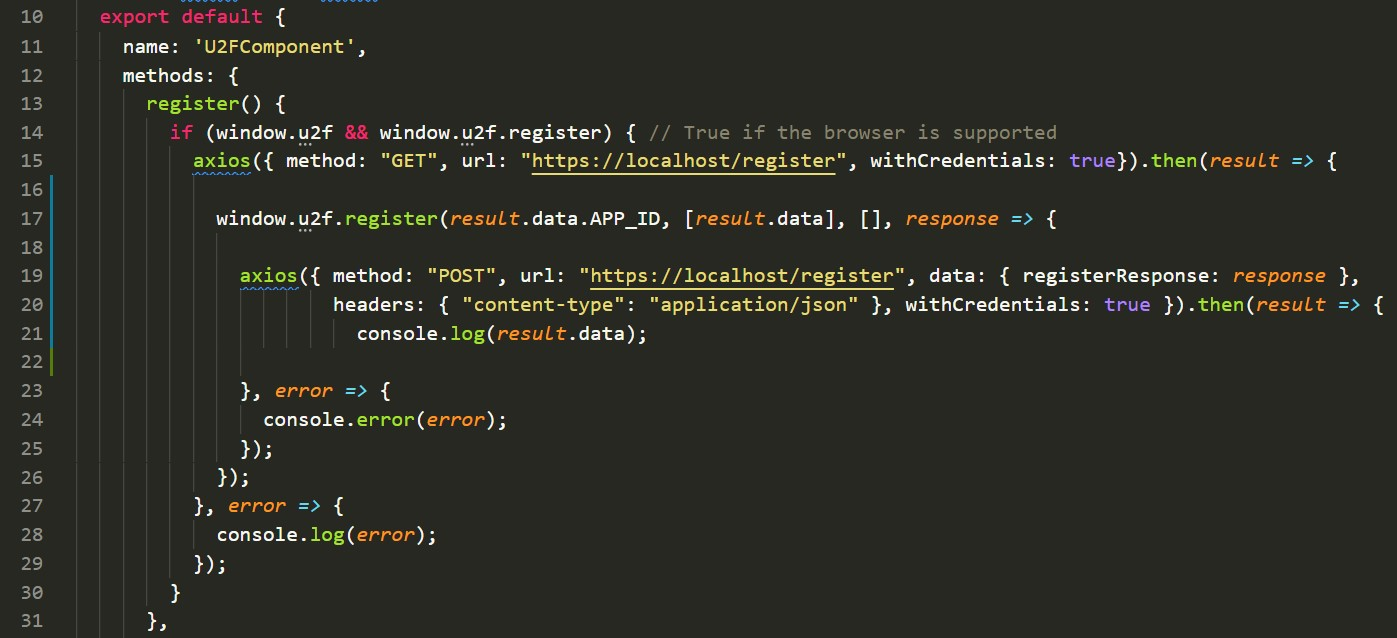
\includegraphics[width=\linewidth]{resources/register-client-code.jpg}
      \caption{Client registration code}
      \label{fig:client-registration}
\end{figure}

The device will the return the Registration Message mentioned earlier. This message contains the user public key, the key Handle, the attestation certificate and the signature over some information (Fig.~\ref{fig:registration-message}). The Registration Message will then be forwarded by the Client to the server, which will use it under the name \texttt{registerResponse}, as seen in Sec.~\ref{server-registration}.

\begin{figure}[h]
    \centering
    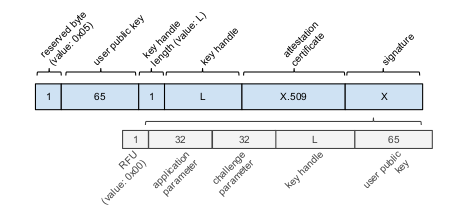
\includegraphics[width=\linewidth]{resources/registration-message.png}
      \caption{Registration Message}
      \label{fig:registration-message}
\end{figure}

\subsubsection{Client Authentication}\label{client-authentication}
Refer to Fig.~\ref{fig:client-authentication}. The pattern is identical to the registration phase. Here, the function \texttt{sign} takes as inputs the web origin (\texttt{result.data.appId}), the challenge (\texttt{result.data.challenge}), and the entire object sent by the server (\texttt{result.data}).

\begin{figure}[h]
    \centering
    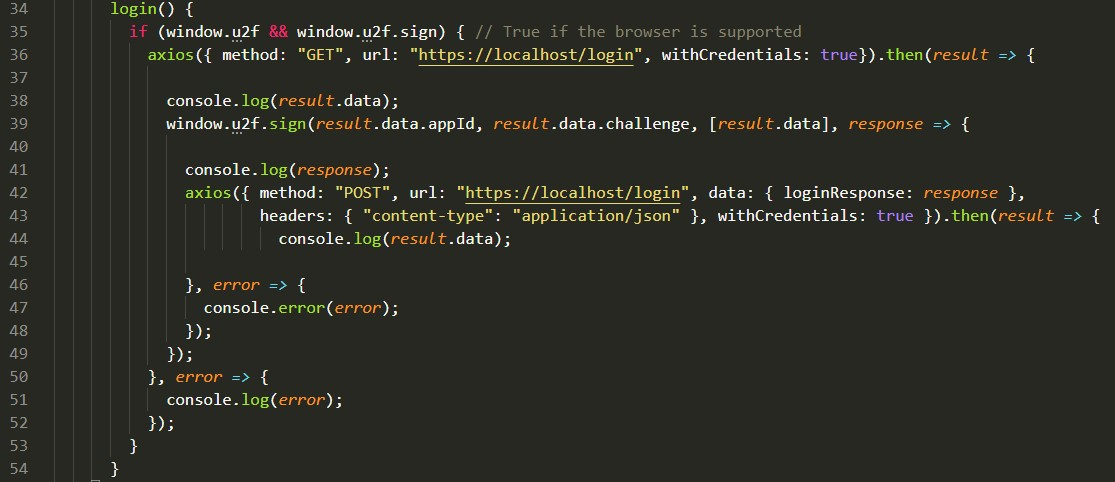
\includegraphics[width=\linewidth]{resources/login-client-code.jpg}
      \caption{Client authentication code}
      \label{fig:client-authentication}
\end{figure}

The security key then returns the Authentication Message mentioned earlier (Fig.~\ref{fig:authentication-message}), which contains the counter and the signature over some parameters, among them the Test of User Presence.

\begin{figure}[h]
    \centering
    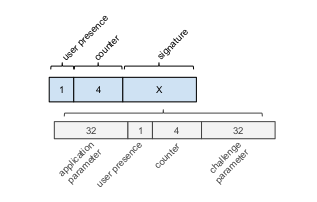
\includegraphics[width=0.5\linewidth]{resources/authentication-message.png}
    \caption{Authentication Message}
    \label{fig:authentication-message}
\end{figure}
\section{Future Work}
As Google says under the Chrome Extension for U2F protocol, \emph{``support for this compiled U2F Chrome extension is being formally deprecated. No further updates or enhancements are planned, and migration to using the support built into Chrome or migration to WebAuthn is recommended''}\footnote{\url{https://github.com/google/u2f-ref-code/tree/master/u2f-chrome-extension}}. This is also the motivation under manually importing the file \texttt{u2f-api.js} into the client-side of my application.

Future works with authentication using security keys should address the standard WebAuthn~\cite{webauthn}.

In addition, this sample can be used as a template for developing meaningful web applications that harness databases and a more complex structure.
\section{Conclusion}
With this report I analyzed in detail the reasons why security keys appear to be more secure than other commonly used second factor technologies.

I outlined how the YubiKey Security Key NFC works under the hood, focusing on the parts of the protocol which are more meaningful from a security and development point of view. I did not analyze the cryptographic standards, as it was not my intention.

Finally, I explained how I used those protocols to develop a small, sample web application, taking also inspiration by a brief tutorial.

My main objective was to show to the reader how convenient is to use a security key, both from the perspective of the user and the developer.

\vspace{12pt}

\bibliographystyle{unsrtnat}
% Cannot upload \bibliographystyle{IEEEtran} with natbib, don't know why
\bibliography{bibliography}

\end{document}
